\documentclass[12pt,a4paper]{ctexart}
\usepackage{titlesec,graphicx,amsmath,amssymb,tikz}
\usetikzlibrary{shapes.geometric,arrows}
\tikzstyle{startstop}=[rectangle,rounded corners,minimum width=1cm,minimum height=0.5cm,text centered,draw=black,fill=red!30]
\tikzstyle{process}=[rectangle,minimum width=1cm,minimum height=0.5cm,text centered,draw=black,fill=orange!30]
\tikzstyle{arrow}=[thick,->,>=stealth]
\graphicspath{{figures/}}
\titleformat{\section}{\normalfont\large\bfseries}{\thesection}{1em}{}
\title{
    {\heiti\zihao{2} 大英四研究过程总结}\\
    {\songti\zihao{4} ————互联网抽象文化与网络暴力之间的关系}
}
\author{
    {\songti\zihao{4} 小组成员: 李维奇林, 潘翰霖, 张硕, 张书恺}\\
}
\date{最后更新: 2025.6.4}

\begin{document}
\maketitle
\tableofcontents
\newpage

\section{研究主要介绍}
\subsection{背景}

关键词: 抽象文化, 网络暴力.

(抽象文化经历一个从直播间推广到社交媒体再到整个网络空间的过程, 起源于一些主播为了吸引粉丝、提高热度而作出奇怪的行为, 发表奇怪的言论.
所谓"黑粉"在抽象文化的最初传播中起到了重要的作用, 将他们内部的风波带进了社交媒体如微博, 形成"黑粉"文化, 他们极力地抹黑网络主播等网红, 也就是对主播实施网络暴力, 并将其塑造成"恶棍"、"坏人", 甚至将其视为"反动分子".
为了躲避网络平台的监管, "黑粉"使用抽象话来模糊各种概念, 创造许多简单但内涵丰富的词汇、缩写, 使得这些梗得以在某些社交媒体中传播.
接着, 更加广大的网络用户开始跟风使用这些抽象话, 他们更多只是单纯地玩文字游戏或者是体现自己的"合群", 而不去考虑抽象话最初的意思.
抽象文化从此走进了最广大网络用户的生活, 人们开始习惯于使用抽象话, 在解读这些话的内涵和说话者想要表达的意思中产生欢乐, 在最常见的场景当中, 抽象话、梗的网络暴力成分被逐渐消解、解构, 这些简短的文字具有极高的"超链接"能力, 可解读的自由度极高, 依靠极弱但是有趣的某些关联性深深印在网络用户的脑海里, 见到这些梗人们便会心一笑.
虽然抽象文化中最本质的最目的性的暴力性质在逐渐减弱, 但是这不影响抽象文化的传播, 它消解了网络暴力的特征(说话者是否隐含暴力成分成为了可选择的因素), 抽象文化寄生在日渐普及的网络空间中, 直接影响着网络用户最常用的语言, 并在一定程度上塑造了网络的文化氛围.
抽象文化的影响力在不断增强.)

最终稿:

抽象文化经历了从直播间发源、向社交媒体扩散、最终渗透至全网空间的传播过程. 本研究旨在揭示当代数字生态中抽象文化与网络暴力的动态博弈关系.

抽象文化最初源于网络主播为吸引流量刻意采用的非常规言行, 其传播则依托"黑粉"群体推动——他们通过在微博等平台发起系统性抹黑行动, 将直播冲突扩大化. 这类攻击行为将攻击对象塑造为"恶人"或"反动派", 形成了一种以公开污名化为核心的新型网络暴力.

为规避内容审查, 黑粉群体开发出抽象话这一语言工具: 通过语义模糊化、隐喻缩写和多义符号实现攻击内容的隐蔽传播. 随着抽象话渗入主流网络文化, 其功能发生本质转变: 普通用户剥离其原始恶意, 将其改造为社交娱乐符号. 典型案例(如"牢大""耄耋(猫爹)"等暴力梗)显示, 广泛传播使这类表达与攻击性脱钩, 转化为中性幽默. 用户对相同短语的差异化解读产生集体娱乐效果, 推动抽象文化深度融入日常网络交流, 重塑了数字文化规范.

\subsection{研究意义}%需要删减

本研究通过揭示数字生态中抽象文化与网络暴力的复杂互动具有重要价值:

演变轨迹溯源: 完整呈现抽象文化从主播刻意挑衅到被黑粉武器化的过程, 阐明社交媒体抹黑如何建构"反派"形象, 形成新型公开羞辱式网暴.

文化转型发现: 核心揭示抽象话进入主流后的本质蜕变——普通用户通过集体再创作剥离其恶意属性, 典型案例证明广泛传播能将其转化为中性娱乐符号.

理论突破: 颠覆“网络暴力内容必然持续有害”的预设, 证明数字社群具有动态重构符号的能力: 展示冲突性亚文化如何通过意义再造成为主流交际规范; 建立"攻击性→文化货币"的转化分析框架.

实践启示: 为平台内容治理提供新思路——区分恶意攻击与娱乐化转用, 制定差异化管控策略.

该研究从根本上推进了对网络文化符号流动性的认知, 揭示了集体诠释如何消解语言暴力, 为理解数字时代的表达嬗变与身份建构提供关键范式.

\subsection{研究的问题}%需要删减

%抽象文化流行的原因与其本身的特点有关吗? (除非问卷能够证明)

普遍的流行与暴力之间似乎存在着一种负增长的关系, 抽象文化流行的背后是消解暴力特征的过程吗?

%各种抽象文化的出现、形式、内容之间有无相似性?

网暴的动机有没有什么相似点?

%利用抽象来进行网暴的同时躲避监管是否是最常见的做法?

%能否给出明确的定义来区分单纯的玩梗与真正的网暴?(无假设)

%怎么反制这些抽象性质的网暴?(无假设)

最终讨论结果详细问题:

鉴于上述关于互联网抽象文化发展的大概背景与网络暴力的定义、性质、影响等,我们课题组希望得到抽象文化与网络暴力二者在发展过程中的程度变化,以及在尽量广泛的网民群体中的影响的关系。我们把这个问题分为三个方面。

首先,因为互联网抽象文化的发展迅速、多元化,得到具有时效性的网络抽象文化的信息框架是必要的,这包括它在网络交流语言中的作用和用以交流的实用性和流通性(流通性主要指在网民群体中的泛用性)两个重要信息,做好这一方面有助于接下来对于抽象文化的分析。

其次,我们需要了解网络暴力的起源,即暴力性语言如何在互联网平台上、在网民的交流中产生,特别是使用抽象网络语言进行的交流,这样,我们可以分析在抽象文化交流的过程中产生的部分网络暴力现象。

然后,接着按时间顺序来看,网络暴力行为将会走出施暴人群的圈子,网络暴力的语言被抽象化,被更多人得知、调侃,暴力性随之消解,我们课题组同样需要分析这一消解的过程。

\subsection{假设}%需要修改

抽象文化的内容之间存在着某种联系, 容易被人熟悉, 这是抽象文化快速传播的原因.

随着这些抽象词汇和表达的流行, 它们的暴力性会不断减弱, 但抽象文化的影响力不会减弱.

抽象文化的内容都经历了一个相似的产生与变革过程.

大部分网暴都源于未知群体与已知个人/群体之间的利益矛盾, 未知群体利用了这个优势.

利用抽象来进行网暴的同时躲避监管是最常见的做法.

\subsection{研究阶段性目标}

抽象文化与网络暴力的定义区分.

抽象文化内容暴力性与流行性的关系.

在抽象文化中产生网络暴力语言的过程.

网络暴力表达的暴力性解构过程.(没时间做, 已删除)

(如何避免网络暴力)

最终实验设计:

我们课题组设计的研究过程是基于上述问题的三个方面,基于可能得到的这三方面特征数据。除去查找文献得到的实验背景——也就是抽象文化定义、性质,网络暴力定义特征——之外,我们的任务还包括问卷调查和用网络爬虫爬取网络数据两方面。

问卷调查实验设计:

设计这一实验的目的是接近广大网民人群,了解受调查者对网络抽象文化的了解程度,以及了解网络暴力在互联网空间中的影响程度,同时,我们添加了询问被调查者对抽象和网暴的认知与见解这一方面,以汇集众智。问卷内容分为三个方面:个人信息(如年龄、地区、接触网络的程度等),抽象梗测试(包含一些流行梗的半开放性测试题),网络暴力测试(包含被调查者被网暴的认知)。

爬取评论区实验设计:

设计这一实验的目的是观察网络空间中,抽象暴力性语言的发展过程。我们课题组打算以几个特定的暴力梗(如牢大,耄耋梗)为重点,并且在特定的网络平台(如bilibili)上观察它们的发展过程。爬虫程序分为四个部分:以网站评论区生成csv数据文件,将数据文件整合为xlsx文件进行统计,暴力梗关键词提取和频率计算,取某些数据生成若干个类型的统计图。

最后,如果实验顺利,我们会从最初仅有定性的认知,到定量地拥有最近的网络抽象文化现状数据以及在抽象文化影响下的网络暴力发展全过程数据,我们会分析这些数据,得出可靠的结论。

实验思路流程图:

\begin{figure}[htbp]
    \centering
    \resizebox{\textwidth}{!}{
        \begin{tikzpicture}[node distance=2cm]
            \node (start)[startstop]{抽象文化与网络暴力};
            \node (process1)[process,below of=start,yshift=0cm,xshift=-3cm]{抽象文化定义、性质等};
            \node (process2)[process,below of=start,yshift=0cm,xshift=3cm]{网络暴力定义、特征等};
            \node (process3)[process,below of=start,yshift=-2cm,xshift=0cm]{抽象文化与网络暴力关系};
            \node (process4)[process,below of=process3,yshift=0cm,xshift=-3cm]{网络暴力的产生过程};
            \node (process5)[process,below of=process3,yshift=0cm,xshift=3cm]{网络暴力的消解过程};
            \node (end)[startstop,below of=process3,yshift=-2cm,xshift=0cm]{分析结果};
            \draw [arrow] (start) -- (process1);
            \draw [arrow] (start) -- (process2);
            \draw [arrow] (process1) -- (process3);
            \draw [arrow] (process2) -- (process3);
            \draw [arrow] (process3) -- (process4);
            \draw [arrow] (process3) -- (process5);
            \draw [arrow] (process3) -- (end);
            \draw [arrow] (process4) -- (end);
            \draw [arrow] (process5) -- (end);
        \end{tikzpicture}
    }
    \caption{研究思路流程图}
    \label{fig:research_process}
\end{figure}
\newpage

\section{研究方法}

\subsection{问卷调查}
%问卷调查方法

\subsection{网络爬虫}
%网络爬虫方法,样本的描述,评估系统的描述
目的: 对互联网中尽量大的区域、尽量多的用户的有关抽象文化或网络暴力的行为进行统计, 设置一系列需要研究的参数指标分类统计.

关键过程: 我们选择bilibili网站上关于耄耋梗内容的图文或者视频下方的评论区, 利用爬虫技术, 获得含有某些人为/主观给定的暴力关键词的评论, 并收集评论者/回复者的一些公开信息, 进行人工分析和机器统计.

使用jieba库得到负面高频词,形成暴力性评分词典,利用原始话题评估词典(根据短语的组合长度区分多级,由于较短的词语更容易出现但与话题的相关度下降)建立基于统计频次的分数评估体系,完成对评论区整体与原始话题相关度的评估;(话题评估体系)

利用jieba与评论暴力度评估词典建立评论区总体攻击性的分数评估体系;(攻击性评估体系)

利用梗词词典建立评估体系,验证采用的数据关联该梗;(梗词评估体系)(略)


\section{研究结果}

\subsection{问卷调查结果呈现}

\subsection{网络爬虫结果呈现}
首先通过梗词关联评估对七个评论区数据进行评估,统计结果如图9所示,七个评论区均能观察到梗词的出现,呈现出与梗的较好关联。这为数据的选取的合理性提供了支撑。

\begin{figure}[htbp]
    \centering
    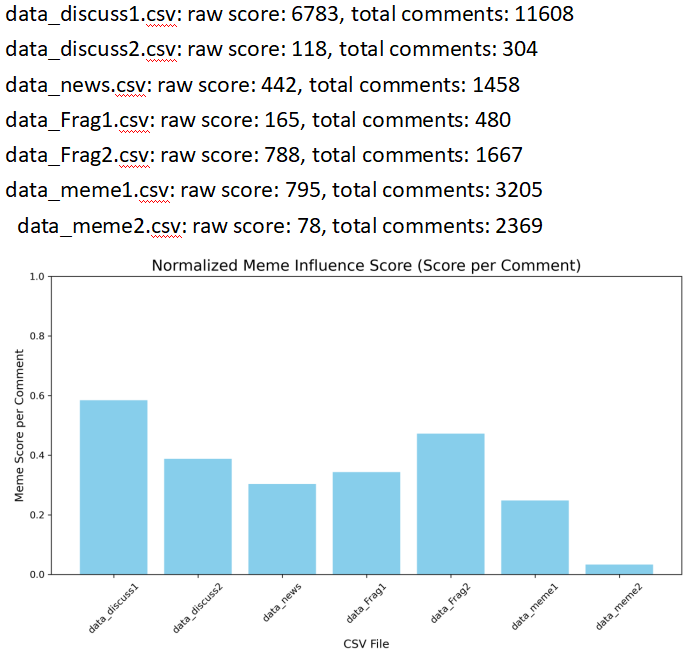
\includegraphics[width=0.8\textwidth]{figures/comment_area_vs_abstract.png}
    \caption{评论区与抽象文化的关联}
    \label{fig:comment_area_vs_abstract}
\end{figure}

接着通过攻击性评估对七个评论区数据进行评估,统计结果如图10所示,可以看到,两个直接讨论流浪猫问题的视频与关于流浪猫新闻的视频的评论区展现出明显更强的攻击性,而两个基于流浪猫问题的二创作品的评论区语言的攻击性明显弱于其他样本。

\begin{figure}[htbp]
    \centering
    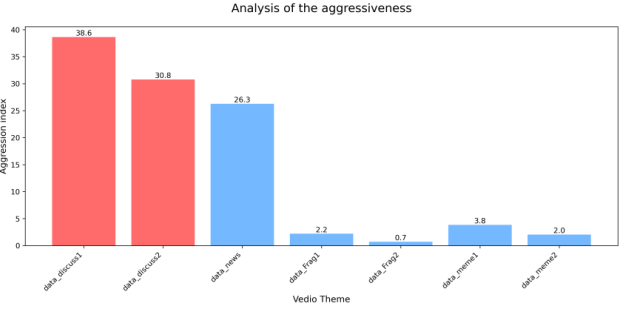
\includegraphics[width=0.8\textwidth]{figures/comment_area_vs_violence.png}
    \caption{评论区与网络暴力的关联}
    \label{fig:comment_area_vs_violence}
\end{figure}

基于攻击性评估对评论区评论攻击性进行评估,根据发布时间统计同日评论的攻击性平均水平,得到评论区攻击性随时间的分布情况。统计结果如图11所示。

\begin{figure}[htbp]
    \centering
    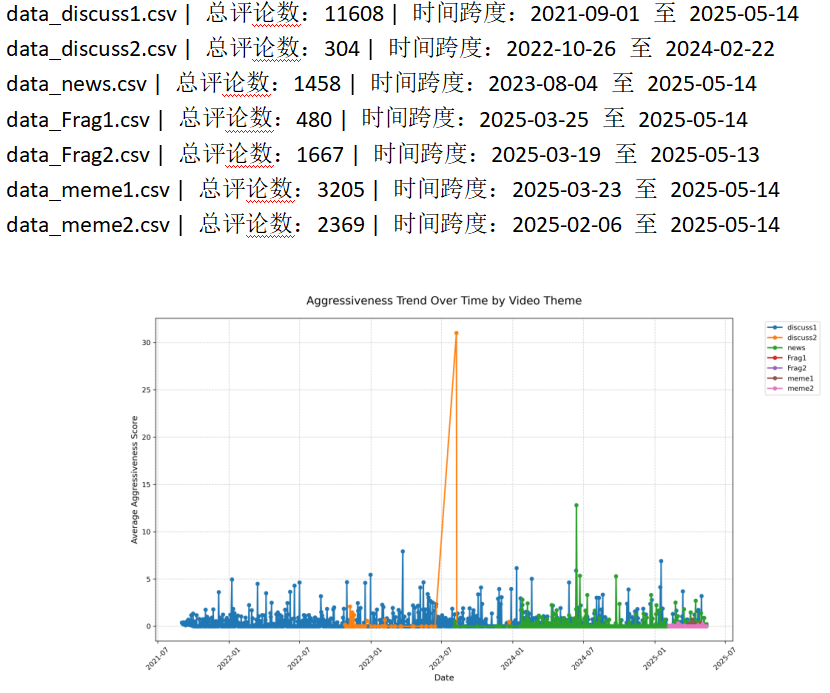
\includegraphics[width=0.8\textwidth]{figures/comment_area_vs_violence_time.png}
    \caption{评论区攻击性随时间的分布}
    \label{fig:comment_area_vs_violence_time}
\end{figure}

关于流浪猫问题讨论的评论区呈现显著的高攻击性,呈现两种不同的表现形式:一个长期处于显著较高的攻击性水平,一个出现远大于其他评论区攻击性水平的高峰值。

关于流浪猫的新闻的评论区呈现较高的攻击性,但是这种攻击性在达到峰值后呈现逐渐下降趋势。

其他作品的评论区攻击性显著较低,且大多不存在较大的波动性。

通过话题相关性评估处理数据,得到统计结果如图12所示,可以看到,从样本“discuss1”到“meme2”评论区的话题相关性呈现下降趋势,这意味着评论区关于流浪猫话题的讨论随着视频主题的偏移出现了明显下降,随着“耄耋”梗的流行,这个词语不再是仅仅谈论流浪猫话题时使用的词汇。

\begin{figure}[htbp]
    \centering
    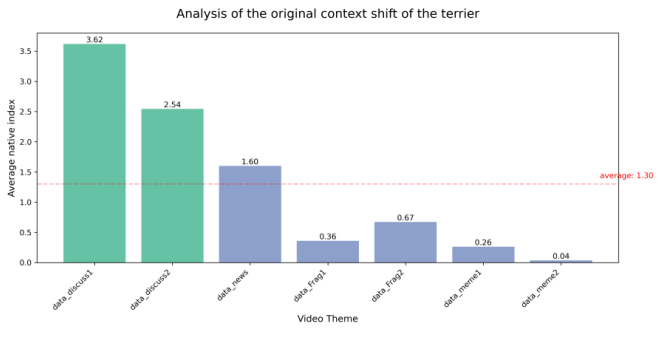
\includegraphics[width=0.8\textwidth]{figures/comment_area_vs_topic.png}
    \caption{评论区与话题的关联}
    \label{fig:comment_area_vs_topic}
\end{figure}

结合主题多样性评估体系,我们对七个评论区的讨论热点进行了提取,得到统计结果如图13所示。

\begin{figure}[htbp]
    \centering
    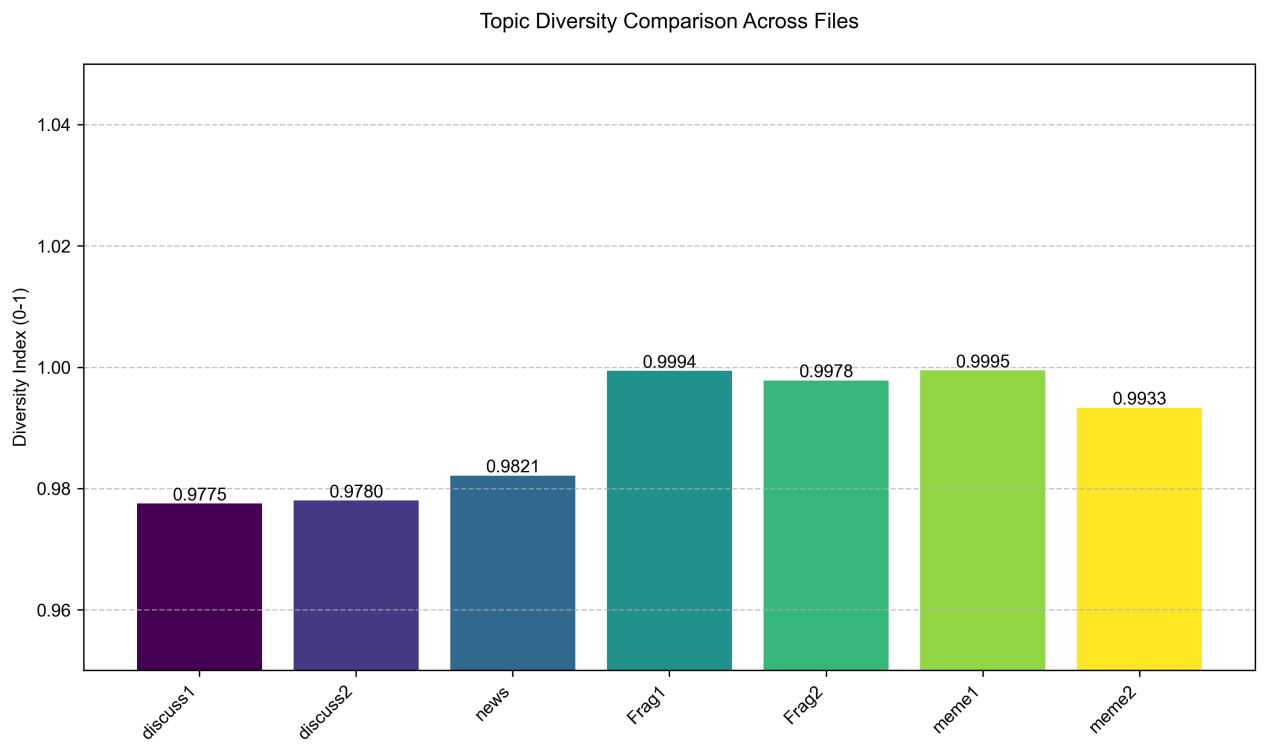
\includegraphics[width=0.8\textwidth]{figures/comment_area_vs_hot_topic.png}
    \caption{评论区与热点话题的关联}
    \label{fig:comment_area_vs_hot_topic}
\end{figure}

关于猫的话题在减少,更多的梗文化如“哈基米”“骇死我力”出现在了评论区,同时攻击性评估得分较高的流浪猫问题讨论类视频在话题多样性上明显得分较低。

实验分析结论:

网络梗词的传播与原始话题的偏移密切相关,随着梗的流行,其语境逐渐脱离原始问题,演变为独立的网络文化现象。

评论区攻击性与话题性质高度相关,严肃社会问题易引发高攻击性讨论,而随着梗词的流行,话题转变向娱乐性更强的非严肃主题,对语言的暴力展现出消解的作用。

关于主题的分析揭示了网络语言从实际问题讨论向多元化、梗文化转变的趋势。

本实验为理解抽象文化对网络语言特性的影响提供了量化支持,同时揭示了网络讨论中攻击性语言的动态变化特征。
\section{Discussion}
%讨论部分
本实验通过对网络空间中网民的各种情况的调查,对抽象文化和网络暴力的关系进行了初步的探索。

抽象文化的流行性在年轻人中具有普遍性,问卷调查的参与者大多对抽象文化有基本了解或比较了解,这说明抽象文化在互联网空间是流行的。我们考虑到了问卷调查具有较大的幸存者偏差,因为接收这份问卷的人更可能是加入了较多圈子、平时有更多空闲时间上网娱乐的人群,因此问卷调查的结果不能说明抽象文化在所有人群中的普及性,但足以说明抽象文化的语言在网络空间传递信息的普遍。

我们注意到,大多数问卷参与者都对抽象文化有较好的了解,但绝大多数人认为自己没有受到或者参与网络暴力,一种可能是很多网民没有意识到一些对自己的抽象的暴力暗示,另一种可能是多数网络暴力是短时间的,经过一段时间后传播成为受众更广、持续时间更长的玩梗行为。

我们做问卷调查时更关注网络人群的行为,而在爬取评论数据时更关注特定抽象现象的发展。我们对有关耄耋梗的视频的评论进行了人工分析,发现在2023年之后,评论的抽象、隐喻程度明显提高,这与抽象文化的流行有关,抽象走出了单一娱乐化的边界,在这些更类似于新闻的视频中,抽象原先的娱乐性被削弱,被网民赋予了更强的讽刺、建政、反思等意义。

具体分析,以样本文件data discuss1和data meme1为例,2023年的评论明显区别于2021年多数评论的风格,评论者更倾向于使用抽象、诙谐的语言,在严肃的社会议题上进行讽刺;2025年后续在这一话题上二创的娱乐视频热度甚至超过2021年,评论的讽刺、隐喻性也明显下降,了解早期事件的是少部分人,而娱乐的人更多了,这符合我们的假设“抽象语言的暴力性随着抽象文化的流行而下降”。


\section{References}
%参考文献部分
%jieba库
%LDA
%代码开源




























%*******原来部分

\section{主要过程记录}

\subsection{预实验(完全没做)}

目的: 检验网络抽象文化的信息相通性, 确定大多数网络用户群体对抽象的认知全能.

关键过程: 在多个平台注册一系列新账号, 以注册时的信息为初始参数, 以账号偏向的抽象范围内的图文、视频等信息的类型为过程参数, 账号活跃一段时间, 判断大数据的推送信息是否跨越不同抽象范围.

\subsection{问卷调查(懒得搬了)}

目的: 研究不同年龄, 性别, 受教育程度的人群对于抽象文化的了解程度以及他们认知中抽象文化与网络暴力之间的关系.

问题: 略

问卷调查结果(粗略分析):

最终参与调查, 提交问卷的人数: 109.

参与者主要位置分布(从多到少): 广东, 山东, 辽宁, 湖北, 北京, 浙江.

参与者年龄段: 15~20岁占57\%, 21~25岁占33\%.

参与者性别: 男$\frac{4}{5}$, 女$\frac{1}{5}$.

参与者受教育程度: 本科占57\%, 普高占23\%.

参与者开始接触网络的大概年龄: 3~6岁占19\%, 6~12岁占61\%, 12~18岁占16\%.

参与者网龄: 2~4年占18\%, 4~8年占52\%, 8年以上占28\%.

上网频率: 时间越长的选项人数越多, 大致呈二次函数递增趋势.

对抽象文化的理解程度: 约$\frac{2}{3}$的人认为自己经常接触抽象文化, 约$\frac{1}{3}$的人认为自己偶尔接触抽象文化。
绝大部分人了解抽象文化, 一半人对自己的了解程度有自信.
图文、视频网站是抽象文化的主要来源.

从抽象文化小测试中, 参与者对大部分有标准情景梗的题目的选择都契合抽象文化实际, 参与者对绝大部分抽象表达的含义理解都有统一性, 印证了抽象文化在网民中的普及性(幸存者偏差).

参与者遭受网络暴力: 是14\%, 否70\%, 不清楚16\%.

认为抽象文化容易引发暴力的参与者数量是认为不容易引发暴力的参与者数量的1.5倍.
他们认为由于抽象文化的解释灵活性、模糊性导致误解是重要原因, 其他还有心态是否严肃、网络空间鱼龙混杂等.
前三个情景, 参与者依分布的选择结果是轻度暴力, 最后一个情景, 参与者依分布的选择结果是中度暴力.

问卷调查结果(完整分析):

图2展示了此次参与问卷调查者的年龄分布,可以看出参与问卷调查者主要集中在15-25岁,即零零后,他们也是网络活动的主要参与者。

\begin{figure}[htbp]
    \centering
    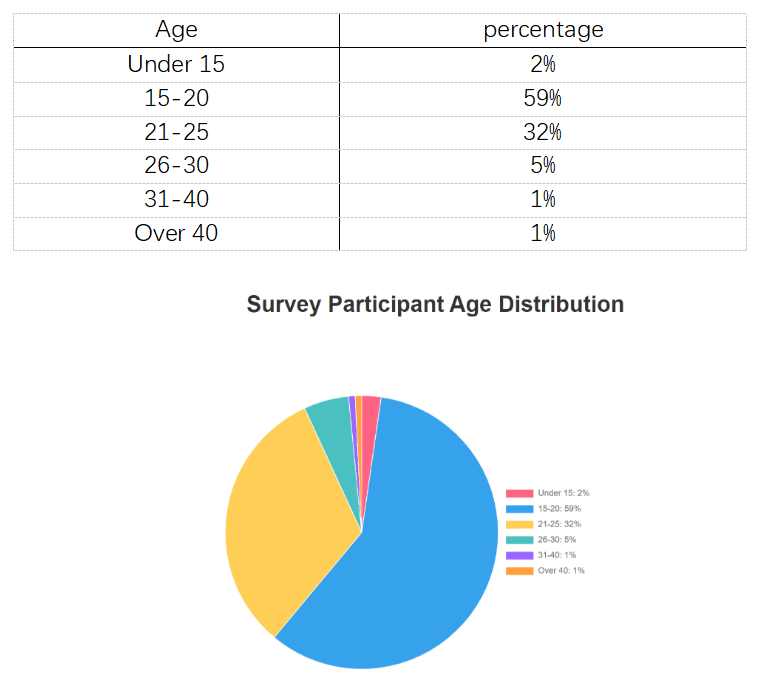
\includegraphics[width=0.8\textwidth]{figures/age_distribution.png}
    \caption{年龄分布}
    \label{fig:age_distribution}
\end{figure}

图3展示了参与调查者第一次使用网络的年龄分布,同时表格2和图表2展示了参与调查者的网龄。可见四分之三的参与调查者在中小学阶段第一次接触网网络,同时四分之三的参与调查者拥有四年及以上网龄,这证明本次问卷调查的对象大多具有比较丰富的网络经验。

\begin{figure}[htbp]
    \centering
    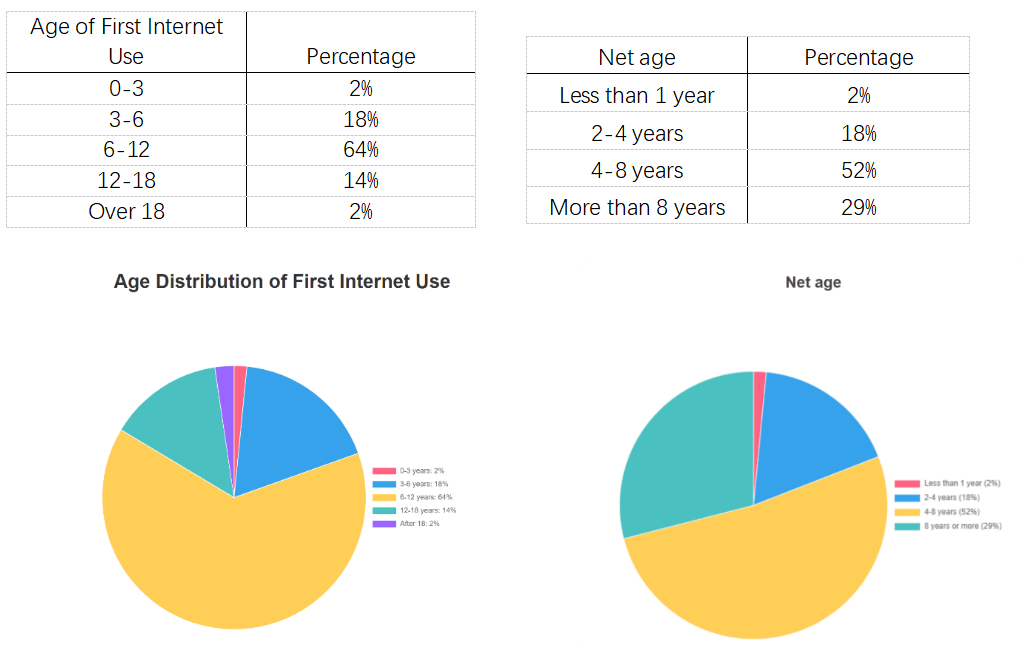
\includegraphics[width=0.8\textwidth]{figures/first_use_age_distribution.png}
    \caption{第一次使用网络的年龄分布}
    \label{fig:first_use_age_distribution}
\end{figure}

图4展示了抽象梗测试部分的回答正确率,参与调查者的正确率分布比较符合正态分布,大部分人对抽象文化有基本了解或比较了解(正确率在30\%至80\%之间),只有小部分人对抽象文化很不了解或非常了解(正确率小于30\%或大于80\%)。可以从中得出抽象文化具有较好的流行性的结论。

\begin{figure}[htbp]
    \centering
    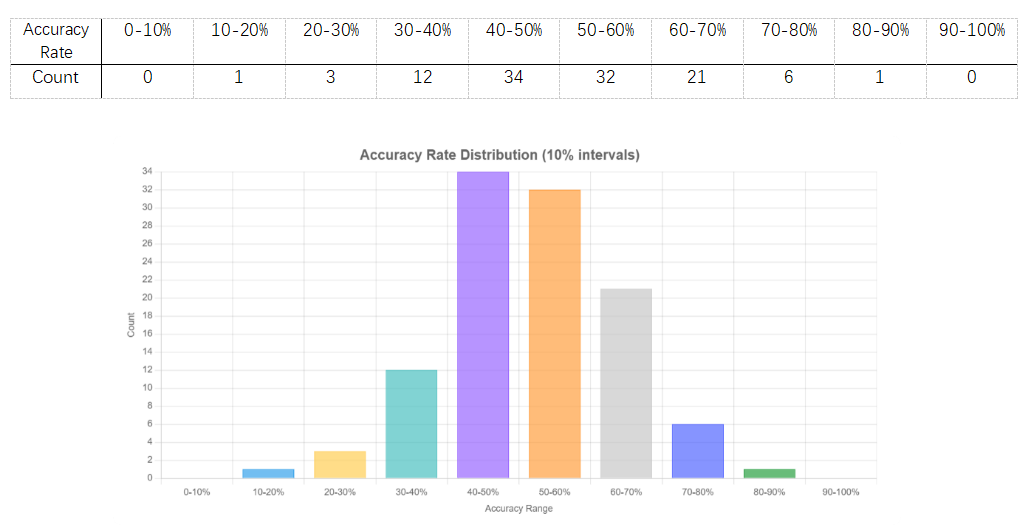
\includegraphics[width=0.8\textwidth]{figures/abstract_test_accuracy.png}
    \caption{抽象梗测试的正确率分布}
    \label{fig:abstract_test_accuracy}
\end{figure}

图5展示了参与调查者正确率和网龄的关系,同时图6展示了参与调查者正确率和第一次使用网络的年龄的关系。忽略样本过少的数据后(样本量少于五个),可见网龄和第一次使用网络的年龄对正确率影响不大,证明抽象文化的流行在年轻人中具有普遍性,无论接触网络的时间长短都可以对抽象文化有一定了解。

\begin{figure}[htbp]
    \centering
    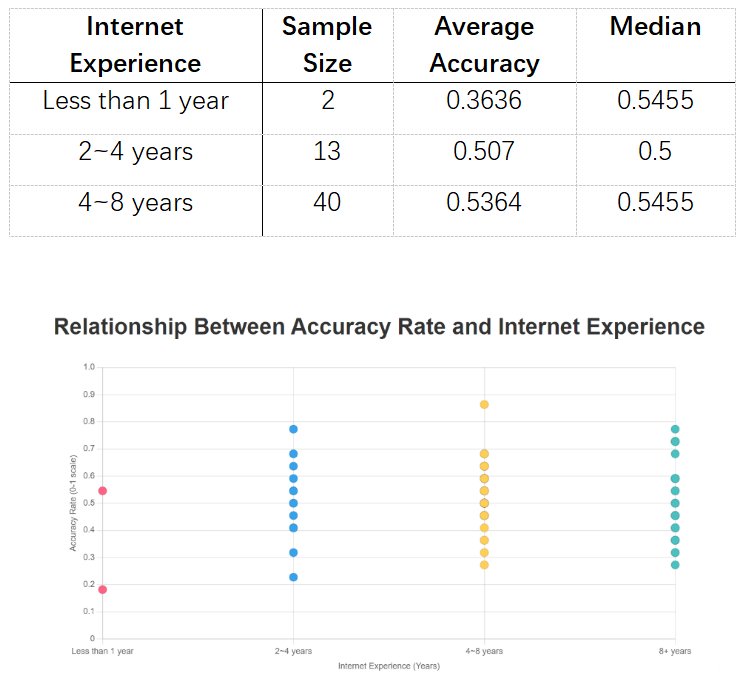
\includegraphics[width=0.8\textwidth]{figures/accuracy_vs_net_age.png}
    \caption{正确率和网龄的关系}
    \label{fig:accuracy_vs_net_age}
\end{figure}

\begin{figure}[htbp]
    \centering
    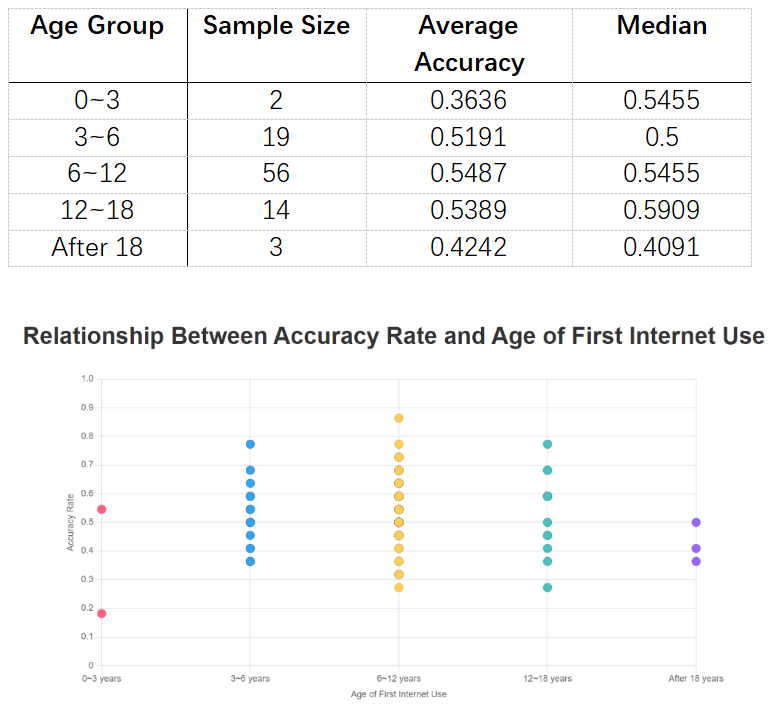
\includegraphics[width=0.8\textwidth]{figures/accuracy_vs_first_use_age.png}
    \caption{正确率和第一次使用网络的年龄的关系}
    \label{fig:accuracy_vs_first_use_age}
\end{figure}

接下来我们分析抽象文化和网络暴力之间的联系。从图7可以看出,超过40\%的人确定抽象文化可能引发网络暴力,只有少部分人不认为抽象文化会导致网络暴力,还有很多人处于中立态度。

\begin{figure}[htbp]
    \centering
    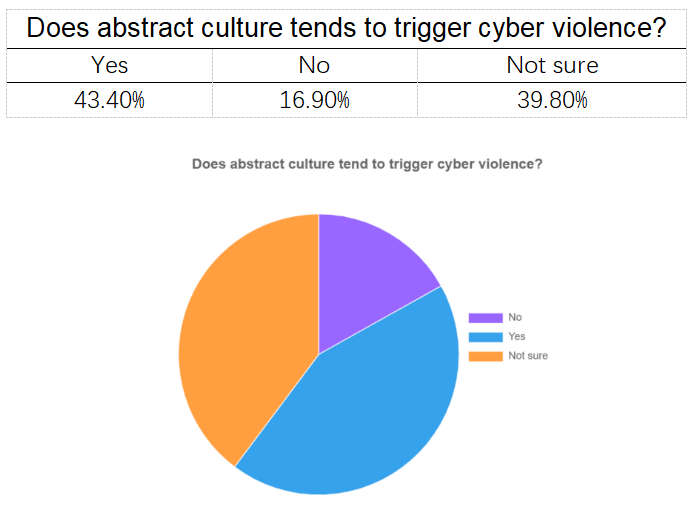
\includegraphics[width=0.8\textwidth]{figures/abstract_vs_net_violence.png}
    \caption{抽象文化与网络暴力的关系}
    \label{fig:abstract_vs_net_violence}
\end{figure}

之后我们做了一个情景假设,模拟抽象文化的方式构建网络对话。以下是情景设计:

Scenario Description (The Chinese text needs to be retained due to the context.)

Scenario 1: Discussion on the gaming forum

A:你这套出装根本不行,实战里就是送人头。

B:你玩过几场啊就在这指点江山?

A:急了?

Scenario 2: Comment section of prank videos

A:第二桶泡面难吃,那为什么不先吃第二桶再吃第一桶呢?

B:不对,我觉得这样第一桶就变成第二桶了。

C:乐子,没看见人家在玩抽象?

Scenario 3: Debate Among Fans of Social Media Stars

A:你家哥哥这演技也能叫好?粉丝滤镜真厚。

B:你行你上啊,键盘侠就会bb。

A:这就急了?(小丑emoji)

Scenario 4: Bickering on the forum

A:废物也就只能躲在屏幕后吠了,现实里敢吭一声?

B:你妈没教你怎么说话是吧?

A:急得开始咬人了?建议回炉重造哦。(微笑emoji)

其中情景1,2反映了日常生活中游戏论坛和一些整活视频的评论区的对话,参与人数较多,流行性较广。情景3,4反映了例如粉丝争论和贴吧互骂的对话,参与人主要是某个特定的小圈子,流行范围有限。 

结果如图8所示,情景1,2都有60\%以上的人认为无暴力或只有轻度暴力,只有不到十分之一的人认为是重度暴力,暴力程度明显较轻;而情景3,4认为达到中度暴力以及重度暴力的人大幅上升,可见暴力程度较重。

从这个情景调查中,我们可以初步得出当流行性增加时抽象文化的暴力程度下降的结论。这与抽象文化的诞生发展相呼应,抽象文化往往在小群体的交流中诞生,带有较强的攻击目的,而广泛传播后人们更关注它的娱乐性,弱化了攻击性。

\begin{figure}[htbp]
    \centering
    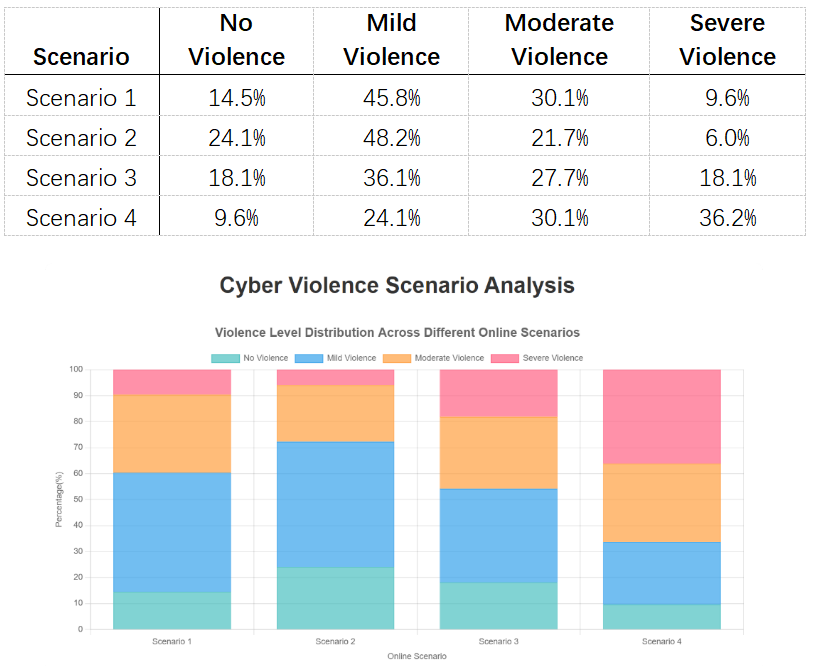
\includegraphics[width=0.8\textwidth]{figures/scenario_vs_net_violence.png}
    \caption{情景与网络暴力的关系}
    \label{fig:scenario_vs_net_violence}
\end{figure}


\end{document}
